\subsubsection{Página Radio}
Esta página web cuenta con una primera sección llamada "Sintonizar una frecuencia" la cual nos permite introducir la frecuencia que deseemos sintonizar en el recuadro blanco. Luego, mediante el botón Sintonizar, podremos sintonizar dicha frecuencia en el Sintonizador FM.

A continuación, se encuentra una sección llamada "Seek", en la cual se encuentran dos botones. El primero, que contiene una flecha hacia arriba, nos permite realizar un SeekUp, es decir, sintonizar una frecuancia mayor con más potencia que la frecuenciaque estuviera sintonizada. De forma análoga, el otro botón, ilustrado medianteuna flecha hacia abajo, nos permite realizar un SeekDown, es decir, sintonizar una frecuencia menor, pero que tenga más potencia que la frecuencia sintonizada en ese momento.

La siguiente sección llamada "Volumen", contiene un slider horizontal que nos permite seleecionar el volumen de la señal de audio. También encontramos un botón de mute, es decir, situar el volumen a 0.

Por último, encontramosla sección "Salida", la cual cuenta con dos botones que nos permiten seleccionar la salida de auido deseada entre Altavoz o Auriculares.

\begin{figure}[h]
    \centering
    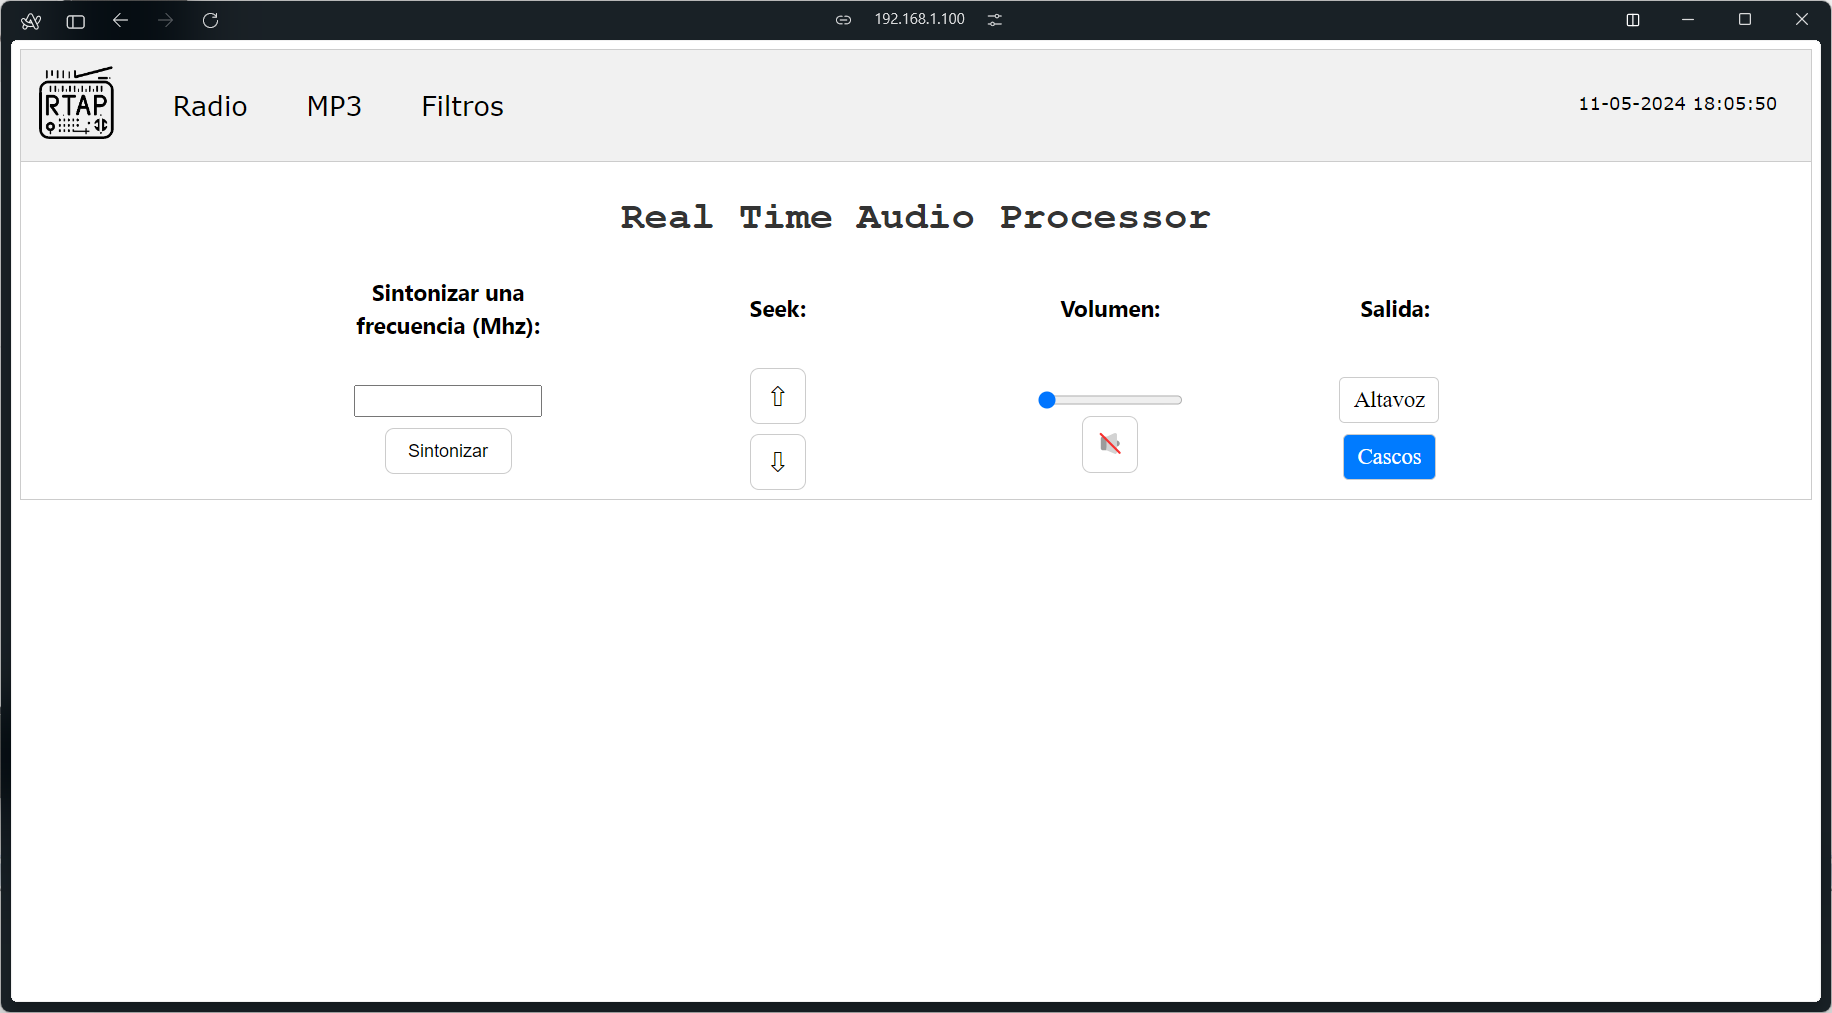
\includegraphics[width=0.6\textwidth]{images/3/3-1/3-1-1-2/Pagina_Radio.png}
    \caption{Página Radio}
    \label{fig:3-1-1-2-Radio}
\end{figure}